\documentclass[oneside]{book}
\usepackage{amsmath}
\usepackage{geometry}
\usepackage{fancyhdr}
\usepackage{graphicx}                   %插入图片
\usepackage{float}                      %图片浮动
\usepackage{lipsum}
\usepackage{xeCJK}                      %调用 xeCJK 宏包
\usepackage{array}
\usepackage{amssymb}                    %\mathbb
\usepackage{ifthen}
\usepackage{yhmath}
\usepackage{amsthm}
\usepackage{enumerate}
\usepackage{siunitx}
\usepackage{hyperref}
\usepackage{unicode-math}
\usepackage[fontsize=8pt]{fontsize}
\setCJKmonofont{LXGW WenKai Mono}
\setmathfont{XITS Math}

\graphicspath{{./pic/}}

\hypersetup{hidelinks, colorlinks=true, allcolors=black, pdfstartview=Fit,breaklinks=true }

\setcounter{secnumdepth}{4} 
\setcounter{tocdepth}{0}

\geometry{papersize={21cm,29.7cm}}
\geometry{left=1.2cm,right=1cm,top=2cm,bottom=3cm}
\setCJKmainfont{STSong} 
\pagestyle{fancy}
% 页眉设置
\fancyhead[L]{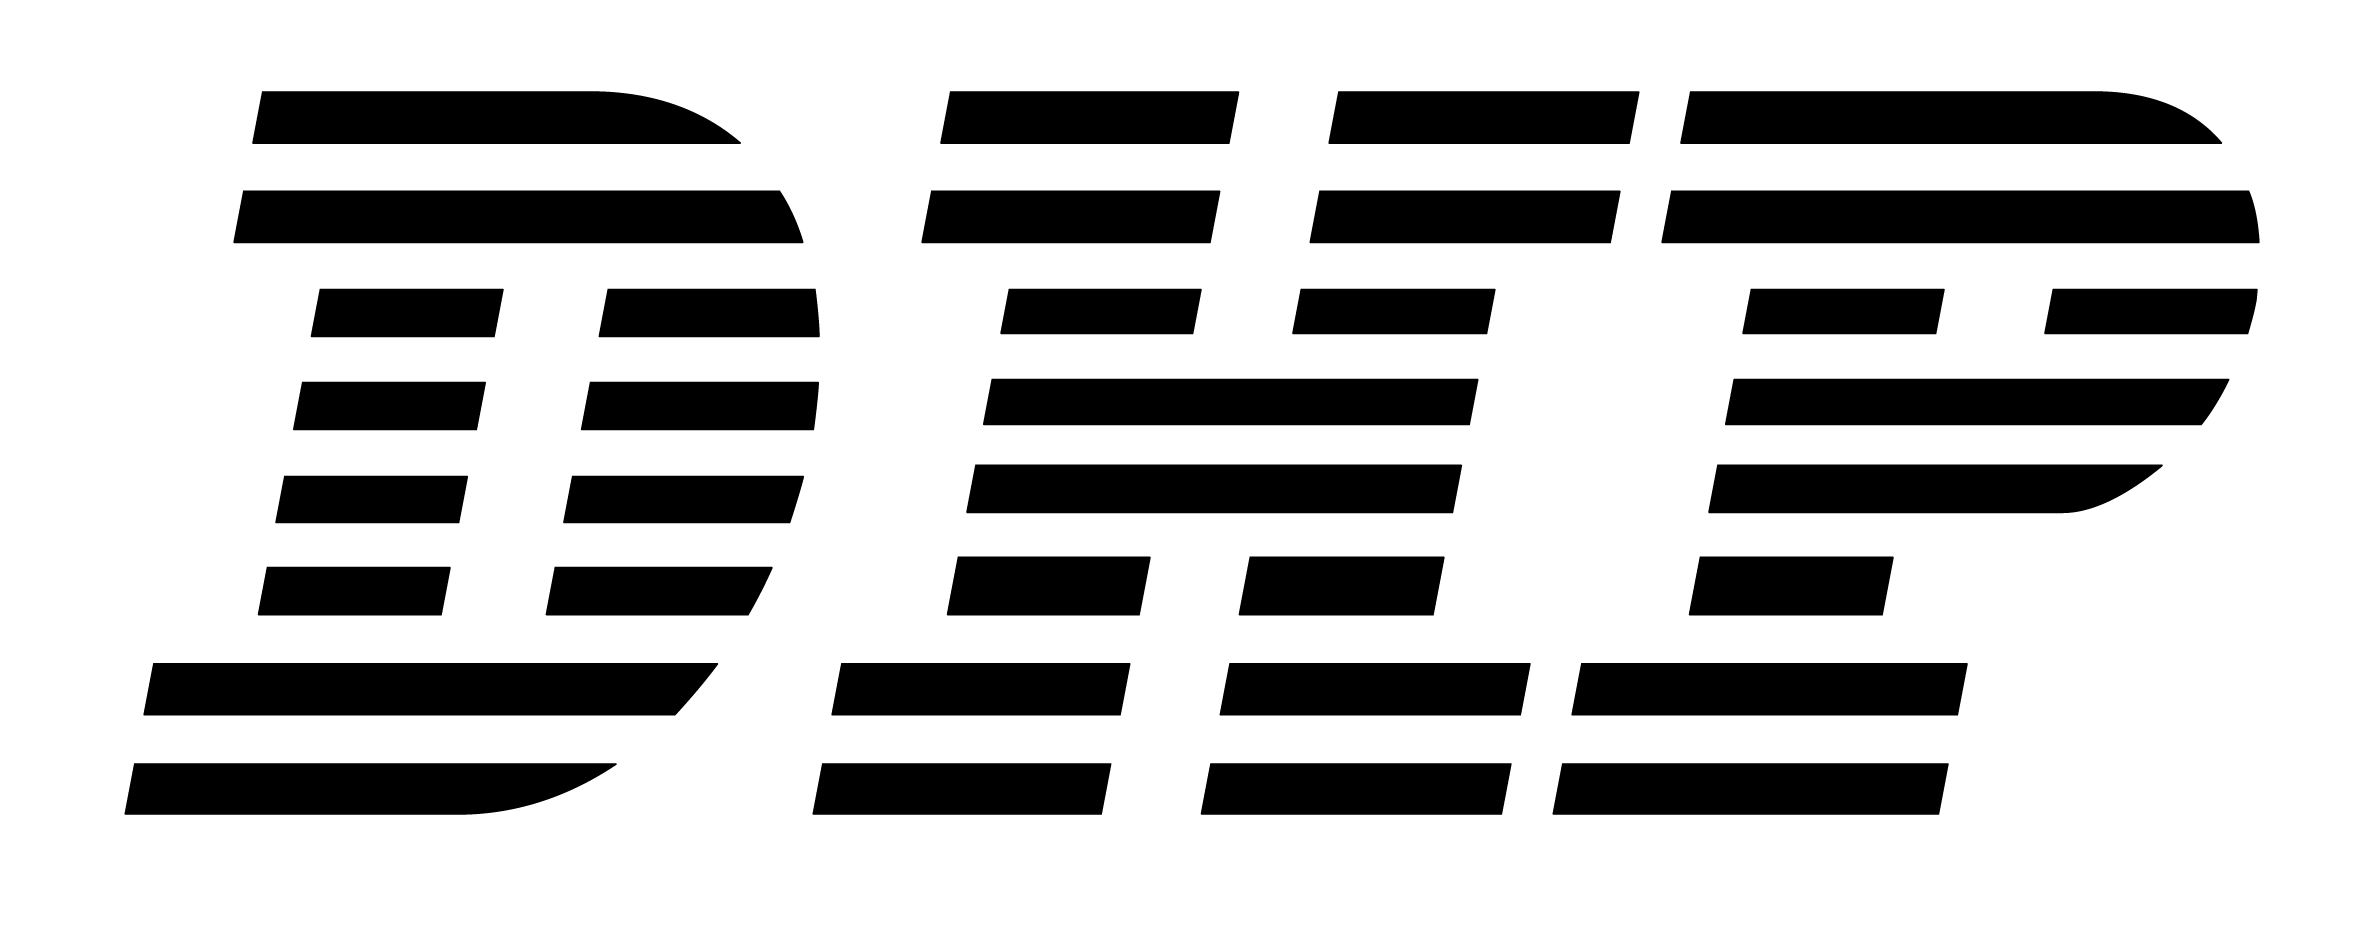
\includegraphics[width=3cm]{DHP.png}}
\fancyhead[R]{Digital Homework Project}

\setlength{\headsep}{1.6cm}             %把正文下移,不会再碰到header
\linespread{1.5}                        %设置行距


\renewcommand{\headrulewidth}{2pt}      % 分隔线宽度0磅
\newcommand{\1}{\underline{\makebox[1cm]{}}}
\newcommand{\2}{\underline{\makebox[2cm]{}}}
\newcommand{\3}{\underline{\makebox[3cm]{}}}
\newcommand{\4}{\underline{\makebox[4cm]{}}}
\newcommand{\blk}{\vspace*{1\baselineskip} }
\newcommand{\blkz}{\vspace*{2\baselineskip} }
\newcommand{\blkx}{\vspace*{4\baselineskip} }
\newcommand{\blkc}{\vspace*{6\baselineskip} }
\newcommand{\blkd}{\vspace*{10\baselineskip} }
\newcommand{\blkv}{\vspace*{16\baselineskip} }
\newcommand{\blkb}{\vspace*{32\baselineskip} }
\newcommand{\brk}{$(\quad \quad)$}
\renewcommand{\qedsymbol}{$\blacksquare$}
\newcommand{\lge}{\large \texttt}
\newcommand{\Lge}{\Large}
\newcommand{\vtr}{\mathbf}
\newcommand{\xl}{\overrightarrow}
\newcommand{\pll}{\kern 0.56em/\kern -0.8em /\kern 0.56em}



%选择题制作
\newlength{\la}
\newlength{\lb}
\newlength{\lc}
\newlength{\ld}
\newlength{\lhalf}
\newlength{\lquarter}
\newlength{\lmax}
\newcommand{\xx}[4]{\\[.5pt]%  
\settowidth{\la}{A.~#1~~~}  
\settowidth{\lb}{B.~#2~~~}  
\settowidth{\lc}{C.~#3~~~}  
\settowidth{\ld}{D.~#4~~~}  
\ifthenelse{\lengthtest{\la > \lb}}  {\setlength{\lmax}{\la}}  {\setlength{\lmax}{\lb}}  
\ifthenelse{\lengthtest{\lmax < \lc}}  {\setlength{\lmax}{\lc}}  {}  
\ifthenelse{\lengthtest{\lmax < \ld}}  {\setlength{\lmax}{\ld}}  {}  
\setlength{\lhalf}{0.5\linewidth}  
\setlength{\lquarter}{0.25\linewidth}  
\ifthenelse{\lengthtest{\lmax > \lhalf}}  {\noindent{}A.~#1 \\ B.~#2 \\ C.~#3 \\ D.~#4 }  {  
    \ifthenelse{\lengthtest{\lmax > \lquarter}}  {\noindent\makebox[\lhalf][l]{A.~#1~~~}%    
    \makebox[\lhalf][l]{B.~#2~~~}%    
    \makebox[\lhalf][l]{C.~#3~~~}%    
    \makebox[\lhalf][l]{D.~#4~~~}}%    
    {\noindent\makebox[\lquarter][l]{A.~#1~~~}%      
    \makebox[\lquarter][l]{B.~#2~~~}%      
    \makebox[\lquarter][l]{C.~#3~~~}%      
    \makebox[\lquarter][l]{D.~#4~~~}}}}




\begin{document}
\tableofcontents


\part{集合与不等式}
    \chapter{集合与逻辑}
        %|数论|集合|14|
        \section{已知$P=\{x|x=4k,k\in \mathbb{Z}\}$, $Q=\{y|y=2k+1,k\in \mathbb{Z}\}$, $R=\{s|s=6k+1, k\in \mathbb{Z}\}$, $a\in P$, $b\in Q$则以下肯定正确的是(\quad \quad)}
        \quad
        \Large{\xx{$a+b\in P$}{$a+b\in Q$}{$a+b\in R$}{$a+b\in P\cap Q\cap R$}}
        \\ \lge{这道题目用Table.}

    \chapter{等式与不等式}
        \section{已知$a$是实数且$a \neq 0$,证明: $\sqrt[]{a^4+\dfrac{1}{a^4}} - \sqrt[]{2} \geq a^2+\dfrac{1}{a^2}-2$.}
        {\large
            \begin{proof}
            欲证明$$\sqrt[]{a^4+\dfrac{1}{a^4}}-\sqrt[]{2} \geq a^2+\dfrac{1}{a^2}-2$$\\
            即证明$$\sqrt[]{a^4+\dfrac{1}{a^4}} \geq a^2+\dfrac{1}{a^2} + \sqrt[]{2} - 2$$\\
            即证明$$a^4+\dfrac{1}{a^4} \geq {(a^2+\dfrac{1}{a^2})}^2 + 2(\sqrt[]{2} - 2)(a^2+\dfrac{1}{a^2})+{(\sqrt[]{2} - 2)}^2$$\\
            即证明$$0 \geq 2 + 2(\sqrt[]{2} - 2)(a^2+\dfrac{1}{a^2}) + {(\sqrt[]{2} - 2)}^2$$\\
            即证明$$0 \geq 2(\sqrt[]{2} - 2)(a^2+\dfrac{1}{a^2})+8 - 4\cdot \sqrt[]{2}$$\\
            即证明$$0 \leq a^2+\dfrac{1}{a^2} + \dfrac{8 - 4\cdot \sqrt[]{2}}{2(\sqrt[]{2} - 2)}$$\\
            即证明$$0 \leq a^2+\dfrac{1}{a^2} - 2$$\\
            因为$$a \in \mathbb{R}, a \neq 0$$\\
            显然$$a^2+\dfrac{1}{a^2} \geq 2$$\\
            因为以上步骤均可逆,\\
            得证.

            \end{proof}
        }
    
        \section{已知$a,b,c$为实数,证明$a^2+b^2+c^2 \geq bc+ca+ab$.}
        {\large
        证:
        \\
        欲证明$$a^2+b^2+c^2 \geq bc+ca+ab$$\\
        即证明
        \begin{align}
            \begin{aligned}
               a^2+b^2+c^2 - bc-ca-ab &\geq 0 
            \end{aligned}
        \end{align}
        $\because$
        \begin{align}
            \begin{aligned}
                a^2+b^2+c^2 - bc-ca-ab &= \frac{1}{2}(2a^2+2b^2+2c^2 - 2bc-2ca-2ab)
                \nonumber\\
                &= \frac{1}{2}((a-b)^2+(a-c)^2+(b-c)^2)
            \end{aligned}
        \end{align}
        显然$$\frac{1}{2}((a-b)^2+(a-c)^2-(b-c)^2) \geq 0$$\\
        $\therefore$ (1)式得证.\\
        $\because$以上步骤均可逆,\\
        得证.\\
        
        \rightline{$\blacksquare$}
        }
        \blk
        \Large 22, 23题的证明都用到了分析法,这是一种由结论推导至条件的方法.除此之外证明不等式的常用方法还有综合法,比较法(做差或做商),以及反证法.
    
        \section{已知实数$a,b,c$满足$a+b+c=0$,且$a>b>c$.求证: $a>0$且$c<0$.}
        {\large
        证:
        \begin{center}
            $\because a>b>c$\\
            $\therefore 3a>a+b+c$\\
            $\because a>c,b>c$\\
            $\therefore a+b>2c$,
            $a+b+c>3c$\\
            $\because a+b+c=0$\\
            $\therefore 3a>0, 3c<0$.\\
            即$a>0, c<0$.
        \end{center}
        }
        \rightline{$\blacksquare$}
        \Large 本题用到了不等式的加法性质,值得注意.
        \blk

        \section{已知$x,y\in \mathbb{R}$,且$x>y$,比较$x^3-y^3$与$xy^2-x^2y$的大小.}
        {\large
            证:\\
            \begin{align}
                \begin{aligned}
                    (x^3-y^3)-(xy^2-x^2y) &= (x-y)(x^2+xy+y^2)-xy(y-x)\nonumber\\
                    &=(x-y)(x^2+xy+y^2+xy)\\
                    &=(x-y)(x^2+2xy+y^2)\\
                    &=(x-y)(x+y)^2\\
                    \because x>y\\
                    \therefore (x-y)(x+y)^2 \geq 0\\
                    \therefore(x^3-y^3)-(xy^2-x^2y) \geq 0.
                \end{aligned}
            \end{align} 
            即$x^3-y^3$大于$xy^2-x^2y$.\\
        }
        \rightline{$\blacksquare$}

        \section{已知$a, b \in \mathbb{R}$, $a - 3b - 5 = 0$, 则$2^a + \frac{1}{8^b}$的最小值是\2.}
        \lge{由条件可得$a - 3b = 5$, 而$2^a + \frac{1}{8^b}$可化为$2^a + \frac{1}{2^{3b}}$, 由基本不等式可得最小值为$8\sqrt{2}$.}

        \section{
            已知$a \in \mathbb{R}$, 函数$f(x)= \log_2{(\frac{1}{x}+a)}$. 
        \\(1) 若$a = 5$, 解 $f(x) \geq 0$;
        \\(2) 若$f(x) - \log_2{((a-4)x +2a -5)} = 0$的解集中仅有一个元素,求$a$的取值范围;
        \\(3) 设$a > 0$,若对任意$t \in [\frac{1}{2}, 1]$, 函数$f(x)$在$[t, t + 1]$上的最大值与最小值的差不超过1, 求$a$的取值范围.
        }
        \begin{enumerate}[(1)]
            \item \lge{因为$\log{2}{(\frac{1}{x}+a)} \geq 0$, 所以$x \in (- \infty, -\frac{1}{x}) $.}
            \item \lge{由$\log_2{(\frac{1}{x}+a)} = \log_2{((a - 4)x + 2a - 5)}$, 变形得$(a-4)x^2 + (a-5)x - 1 = 0$(式1), 且$\frac{1}{x} + a \geq 0$.
                \\若$ a = 4 $, 则$ x = -1$,符合题意;
                \\ $\Delta = a^2 - 6a + 9$ , 解得若$\Delta = 0$,则$a = 3$; 若$\Delta > 0$,则$a \neq 3$; 若$\Delta < 0$,则 $a \in \emptyset$;
                \\若$a = 3$, 则$x = -1$,符合题意;
                \\若$a \notin \{3, 4\}$, 由求根公式得$x_1 = -1, x_2 = \frac{1}{a-4}$;
                \\若$x = -1$是解, 代入到式1中得$\begin{cases} -1 + a > 0 \\ 2a - 4 \leq 0\end{cases}$,解得$a \in (1, 2]$;
                \\若$x = \frac{1}{a-4}$是解, 代入到式1中得$\begin{cases} 2a - 4 > 0 \\ -1 + a \leq0\end{cases}$,解得$a \in \emptyset$;
                \\综上, $a \in (1, 2]\cup \{3,4\}$.
            }
            \item \lge{
                由复合函数单调性的性质可知$f(x)$在$\mathbb{D}$上单调减.
                \\由$f(t)-f(t+1) \leq 1$可得$\log_2{\frac{\frac{1}{t}+a}{\frac{1}{t+1}+a}} \leq 1$;
                \\进一步化简可得$\frac{1}{t} + a \leq 2(\frac{1}{t+1}+a)$,得$\frac{1 - t}{t(t+1)} \leq a$;
                \\令$r = t -1$, 则$r \in [0, ]$; 原式化为$\frac{r}{r^2 - 3r + 2} \leq a$;
                \\若$r = 0$, $a \geq 0$;
                \\若$r \in (0, \frac{1}{2}]$, 原式继续化为$\frac{1}{r+\frac{1}{r}-3 \leq a}$, 由基本不等式解得$a \geq \frac{2}{3}$.
                \\综上, $a \in [\frac{2}{3}, +\infty]$.
            } 
            \end{enumerate}



\part{函数}


    \chapter{函数的性质与应用}
        %|图像|图像变换|函数|对数函数|
        \section{要得到$y = \log{(3-x)}$的图像,只需要作$y = \log{x}$关于$y$轴对称的图像,再向\2平移个单位而得到. }
        \blk

        %|函数单调性|最值|10
        \section{如果$a>0$,设函数$f(x)=\dfrac{2009^{x+1}+2007}{2009^x+1}+\sin{x},x \in [-a,a]$的最大值为$M$,最小值为$N$,那么$M+N=$\2.}
        \blkc

        %|函数|周期性|图像|根|交点|16
        \section{设$f(x)$是定义在$\mathbb{R}$上的偶函数,且$f(2+x)=f(2-x)$,当$x \in [-2,0]$时, $f(x)={\left(\dfrac{\sqrt{x}}{2}\right)}^x-1$,若在区间$(-2,6)$内的关于$x$的方程$f(x)-\log_a (x+2)=0 (a \ge 0 $且$ a \neq 1)$恰有$4$个不同的实数根,则实数$a$的取值范围是$(\quad \quad)$.}
        \quad
        \xx{$(-\frac{1}{4},1)$}{$(8,+\infty)$}{$(1,8)$}{$(1,4)$}
        \blkc

        %|函数|定义域|
        \section{函数$f(x)=\dfrac{\log_2(x-1)}{\sqrt{|x-2|-1}}$的定义域为\3.}
        \blk

        %|函数|二元|值域|条件 
        \section{设$x \geq 0$, $y\geq 0 $, $x+2y=1$,则函数$\omega = 3y^2+2x$的值域为\3.} 
        \blkz

        %|函数|单调性|参数|
        \section{设函数$f(x)=\log_{\frac{1}{2}}(kx^2-2x+5)$在$[-1, 2]$上严格增,则实数$k \in$\3.}
        \blkz
        
        %|函数|值域|参数|
        \section{已知函数$f(x)=\lg(2^x+x^{-x}+a-1)$的值域为$\mathbb{R}$,则实数$a$的取值范围是\3.}
        \blkx
        
        %|二次函数|解集|根个数|
        \section{设二次函数$f(x)=ax^2+bx+1$,且$f(1)=0$,若不等式$f(x) \geq 0$的解集为$\mathbb{R}$,则方程的实根个数为\2.}
        \blkx
        
        %|函数|单调性|对称|恒成立|
        \section{已知函数$y=f(x)$是定义在$\mathbb{R}$上的增函数,函数$y=f(x-1)$的图像关于点$(1,0)$对称.若对任意的$x,y\in \mathbb{R}$,不等式$f(x^2-6x+21)+f(y^2-8y)<0$恒成立,则当$x>3$时, $x^2+y^2$的取值范围是\3.}
        \blkc
        
        %|函数|绝对值|不等式|恒成立|取值范围|
        \section{设函数$f(x)=x|x-a|, a\in \mathbb{R}$.当$x\in [\dfrac{1}{2},2]$时,不等式$f(x)\leq 2$恒成立,试求实数$a$的取值范围.}
        \newpage
        
        %|函数|最值|区间|不等式|恒成立|
        \section{已知定义在区间$[0,2]$上的两个函数$f(x)$和$g(x)$,其中$f(x)=x^2-2ax+4, a\geq 1, g(x)=\dfrac{x^2}{x+1}$.\\(1)求函数$y=f(x)$的最小值$m(a)$;\\(2)若$\forall x_1, x_2\in [0,2]$, $f(x_2)>g(x_1)$恒成立,求$a$的取值范围.}
        \blkc

        %|函数|三次|区间|最值|
        \section{已知函数$f(x)=2x^3-3x^2+2$,求函数$f(x)$在区间$[-1, 2]$上的最大值.}

        \section{已知$f(x)$是定义在$[-1,1]$上的减函数,且$f(x-1)<f(1-3x)$,则$x$的取值范围是\2.}
        \lge{这种题目得考虑自变量在定义域内,再求解.}
        
        \section{已知函数$f(x)=4+log_a(2x-3),(a>0\wedge a\neq 1) $的图像恒过定点$P$,且点$P$在函数$g(x)=x^a$的图像上,则$a=$\3.}
        \lge{这边定点求错了.}
        
        \section{已知函数$f(x)=|x-1|(x+1),x\in [a,b]$的值域为$[0,8]$,则$a+b$的取值范围是\3.}
        \lge{图是画对了的,但是脑子卡住了,关于值域没反应过来.}
        
        \section{已知奇函数$f(x)$是定义在$(-2,2)$上的减函数,若$f(m-1)+f(2m-1)>0$,则实数$m$的取值范围是\3.}
        \lge{这题跟26号套路一样一样的,只是增加了对奇函数性质的考察.}
        
        \section{函数$g(x)$对$\forall x \in \mathbb{R}$,有$g(x)+g(-x)=x^2$,设函数$f(x)=g(x)-\dfrac{x^2}{2}$,且$f(x)$在区间$[0,+\infty)$上增,若$f(a)+f(a^2-2)\leq 0$,则实数$a$的取值范围是\3.}
        \lge{本题难点在对于$g(x)+g(-x)=x^2$的运用.}
        
        \section{已知函数$f(x)=\begin{cases}(a-0.5)(x-1),\quad \quad x<1\\-x^2-ax+2a+1,\quad x\geq 1\end{cases}$在$\mathbb{R}$上是减函数,则$a$的取值范围是\2.}
        \lge{一通分析后得出不等式组$\begin{cases} a-\frac{1}{2}<0 \\ -\frac{a}{2}\leq 1 \\ a\leq 0\end{cases}$,很多人会忽略最下面一个不等式.}
        
        \section{已知函数$f(x)=\begin{cases} |log_5(1-x)|\quad x<1 \\ -(x-2)^2+2 \quad x \geq 1 \end{cases}$,则方程$f(x+\frac{1}{x}-2)=a,(a\in \mathbb{R})$的实根个数不可能为(\quad \quad).}
        \quad
        \Large{\xx{5个}{6个}{7个}{8个}}\\
        \lge{比较变态的一道题,听说需要分很多类.}
        
        \section{已知函数$f(x)=2x|x+a|-1$有三个不同的零点,则实数$a$的取值范围是\3.}
        \lge{移项化成关于a的等式,画图,数个数.}
        
        \section{已知函数$f(x)$的定义域为$\mathbb{R}$,且$f(x)\cdot f(-x) =1$和$f(1+x)\cdot f(1-x)=4$对$\forall x\in \mathbb{R}$恒成立.若当$x\in [0.1]$时, $f(x)$的值域为[1,2],则当$x \in [-100,100]$时,函数$f(x)$的值域为\3.}
        \lge{对于这题,要进行一个定义域的外延.}

        %|函数|周期性|零点|三角函数|对数函数|16|
        \section{对于函数$f(x)=\begin{cases}\sin\pi x,\quad \quad x\in [0,2]\\0.5f(x-2),x\in (2,+\infty)\end{cases}$,有下列2个命题:\\命题$p$: $\forall x\in (0,+\infty)\Rightarrow f(x)\leq \dfrac{1}{x}$;\\命题$q$:函数$y=f(x)-\ln(x-1)$有$3$个零点,则下列判断正确的是(\quad \quad)}
        \quad
        \Large{\\A.\quad{$p$是真命题,$q$是真命题;}\\ B.\quad{$p$是假命题,$q$是假命题;}\\ C.\quad{$p$是真命题,$q$是假命题;}\\ D.\quad{$p$是假命题,$q$是真命题.}}
        \\ \lge{我们先判断命题$p$,可见$x=2.5$时有极大值,带入发现矛盾,故命题$p$为假.然后判断命题$q$,先画出$f(x)$的图像,然后画出$y=\ln(x-1)$的图像.用计算器求解得分别在$x=1.39,x=2,x=2.6$时有零点,故有$3$个零点,命题$q$成立.}

        %|函数|单调性|解|11|
        \section{已知函数$f(x)=\begin{cases} x^2+(4-3a)x+3a, x<0 \\ log_a(x+1)+1, \quad \quad x\geq 0 \end{cases} (a>0\wedge a\neq 1)$在$\mathbb{R}$上减,且关于$x$的方程\\$|f(x)|=2-x$恰有两个不相等的实数解,则$a$的取值范围是\4.}
        \lge{要仔细考虑$x^2+(4-3a)x+3a$和$|f(x)|=2-x$相切时的情况.}

    \chapter{导数}
        %|三次函数|最值|导数|11 
        \section{若函数$f(x)=x^3-3x$在区间$(a,6-a^2)$上有最小值,则实数$a$的取值范围是\2.} 
        \blkc
    
    \chapter{导数大题}
        %|函数|切线|根个数|恒成立|21
        \section{已知函数$f(x)=mx-\dfrac{m}{x}, g(x)=2\ln x$. \\(a)当$m=2$时,求曲线$y=f(x)$在点$(1, f(1))$处的切线方程; \\(b)当$m=1$时,判断方程$f(x)=g(x)$的实根个数; \\(c) 若$x \in (1, e]$时,不等式$f(x)-g(x)<2$恒成立,求实数$m$的取值范围.}



\part{三角,复数与向量}

    \chapter{三角}
        \section{三角形$ABC$的外心为$O$, 三个内角$A, B, C$所对的边分别为$a, b, c$, $ \xl{AO} \cdot \xl{BC} = \frac{1}{2}a(a-\frac{8}{5}c), b = 4$,则三角形$ABC$面积的最大值为\2.}
        \lge{由外心的性质可知, $\xl{AO} \cdot \xl{BC} = \xl{AO}(\xl{AC}-\xl{AB}) = \xl{AO} \cdot \xl{AC} - \xl{AO} \cdot \xl{AB} = \frac{1}{2}|\xl{AC}|^2 - \frac{1}{2}|\xl{AB}|^2 = \frac{1}{2}b^2 - \frac{1}{2}c^2$, 于是$
        \frac{1}{2}b^2 - \frac{1}{2}c^2 = \frac{1}{2}a^2 - \frac{4}{5}ac$}

        \section{水域养殖水产, $AO, BO$为直线岸线, $OA = 1000$m, $OB = 1500$m, $\angle{AOB} = \frac{\pi}{3}$水域边界为某圆的一段弧$\wideparen{AB}$, 过$\wideparen{AB}$上一点按线段$PA$和$PB$修养殖网箱,知$\angle{APB} = \frac{2\pi}{3}$.
        \\(1) 求岸线上$A$与$B$之间的距离;
        \\(2) 若$PA$上每米40元利润,$PB$上每米30元利润,记$\angle{PAB} = \theta$, 则两段最大经济收益是?(精确到元).
        }

        \begin{minipage}[b]{0.65\linewidth}
            \hfill
            \begin{enumerate}[(1)]
                \item \lge{由余弦定理得$|AB| = 500\sqrt{7}$m.}
                \item \lge{由正弦定理得$\frac{PA}{\sin\theta} = \frac{PA}{\sin(\frac{\pi}{3}-\theta)} = \frac{500\sqrt{7}}{\sin\frac{2\pi}{3}}$, 设$\frac{500\sqrt{7}}{\sin\frac{2\pi}{3}} = c$,则$PA = c \sin(\frac{\pi}{3}-\theta)$, $PB = \sin\theta$, 利润为$40c\sin(\frac{\pi}{3}-\theta) + 30c\sin\theta$, 化简可得$10c(2\sqrt{3}\cos\theta + \sin\theta)$, 使用辅助角公式可得$10\sqrt{13}c\sin(\theta + \arctan 2\sqrt{3})$, 求得最大值为16166元.}
            \end{enumerate}
            \end{minipage}
            \hfill
            \begin{minipage}[b]{0.25\linewidth}
            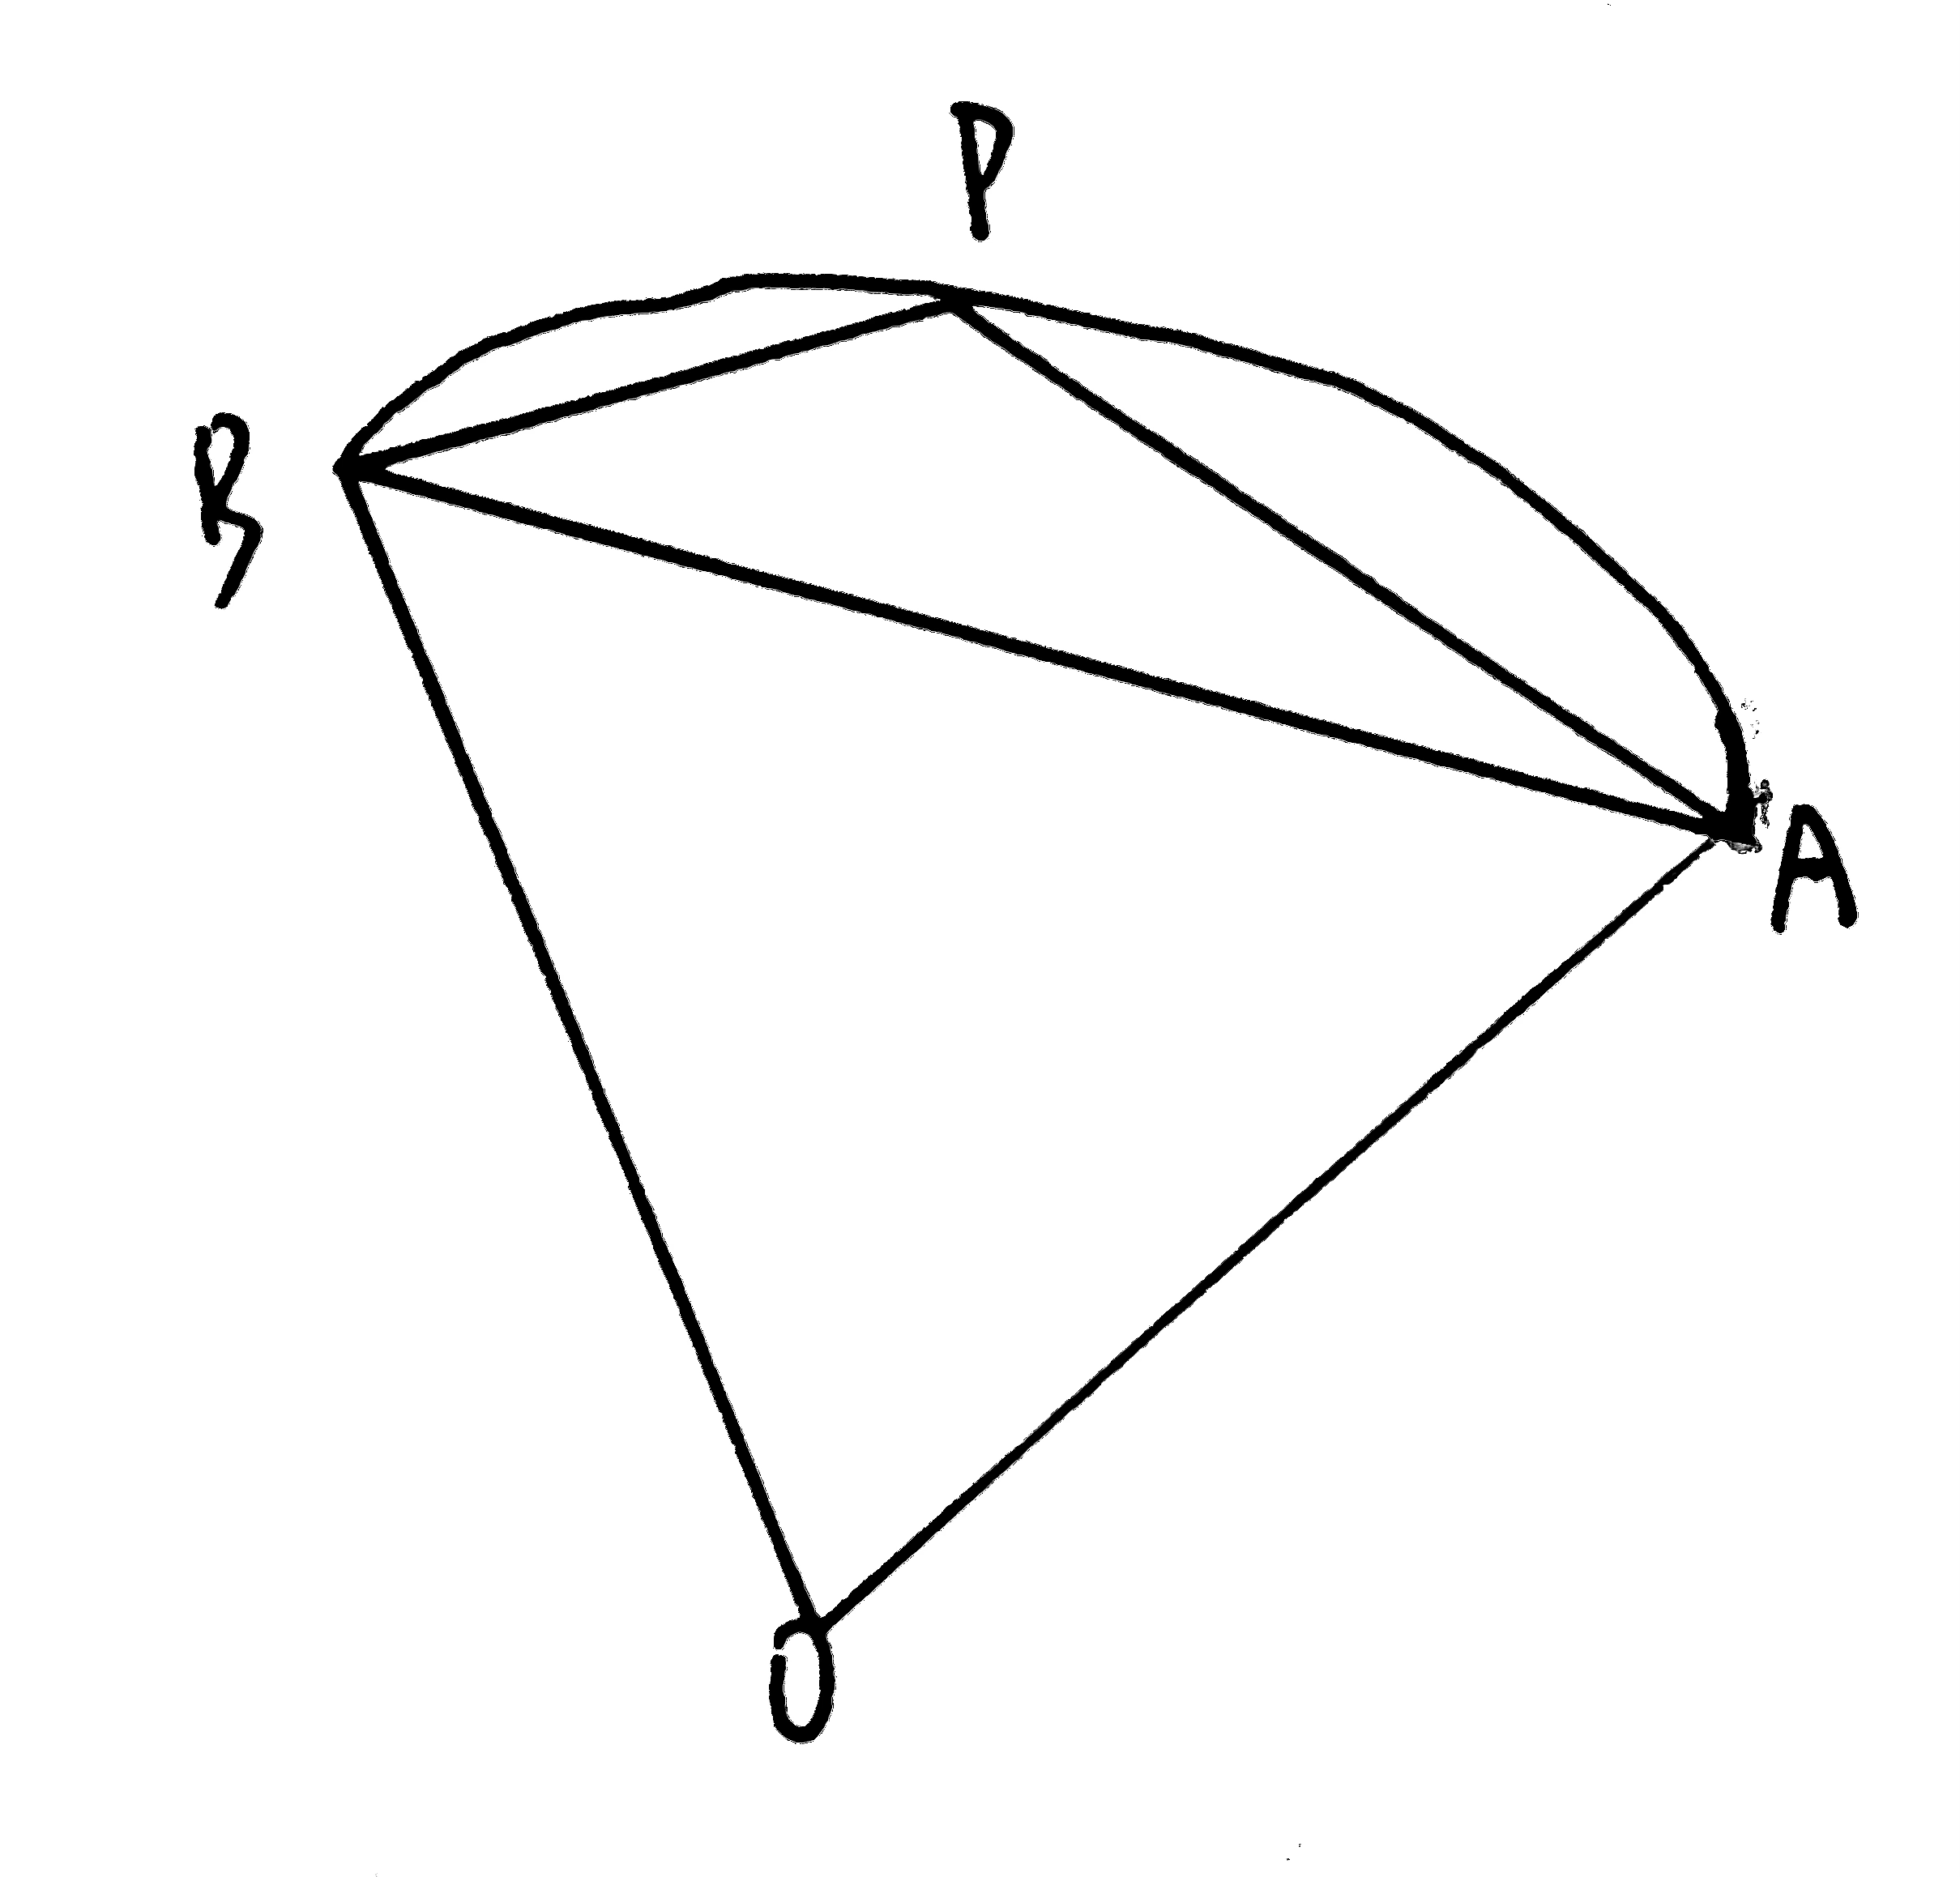
\includegraphics[height=85pt]{1.png}
        \end{minipage}

    \chapter{向量}
        %|向量|10|
        \section{已知平面向量$\mathbf{a},\mathbf{b},\mathbf{c}$满足$|\vtr{a}|=|\vtr{b}|=\vtr{a}\cdot \vtr{b}=2$,且$(\vtr{b}-\vtr{c})\cdot(3\vtr{b}-\vtr{c})$,则$|\vtr{c}-\vtr{a}|$最小值为\3.}
        \blkc


\part{几何体与空间几何}

    \chapter{立体几何}
        %|立体几何|异面角 
        \section{在如图的长方体中, $AD=AA_1=1, AB=2$,点$E$在棱$AB$上移动,求异面直线$AC_1$与$A_1D$所成角的余弦值.} 
        \blkx




\part{概率与统计}

    \chapter{计数原理}
        %|二项式定理|二项展开式|5 
        \section{$(2x+1)^{10}$的二项展开式中第八项为\2} 
        \blk

    \chapter{概率初步}
        \section{把一个骰子连续抛掷两次, 记事件$M$为``两次所得点数均为奇数'', $N$为``至少有一次点数是5'',则$P(N | M = )$\2.}
        \lge{我们知道$P(N|M) = \frac{P(M)}{P(MN)} = \dfrac{\dfrac{3 \times 3}{36}}{\dfrac{1 + C_2^1C_2^1}{36}} = \frac{5}{9}$.}

        %|概率|19 
        \section{某超市在节日期间进行有奖促销,凡在该超市购物满$400$元的顾客,将获得一次摸奖机会,规则如下:
        奖盒中放有除颜色外完全相同的$1$个红球, $1$个黄球, $1$个白球和$1$个黑球,顾客不放回的每次摸出$1$个球,若摸到黑球则停止摸奖,
        否则就继续摸球,规定摸到红球奖励$20$元,摸到白球或黄球奖励$10$元,摸到黑球不奖励. 求$1$名顾客摸球$2$次停止摸奖的概率.}
        \blkx

        %|统计|概率|
        \section{在一次抽奖活动中,假设每10张奖券中有一等奖券1张,可获价值50元的奖品;有二等奖券3张,每张可获得价值10元的奖品;其余6张没有奖.某顾客从这10张奖券中任抽2张,求该顾客获奖的概率.}
        \blkc

        %|概率|8|互斥|
        \section{事件$A$与事件$B$互斥,它们都不发生的概率是$\dfrac{3}{5}$,且$P(A)=2P(B)$,则$P(\overline{A}) $\2.}
        \lge{互斥意味着两件事不可能同时发生.则仅发生$A$或发生$B$的概率为$1-\dfrac{3}{5}=\dfrac{2}{3}$.接下来就很方便了.}

    \chapter{统计}
        %|统计|最小二乘法|回归|
        \section{已知一组数据点$(x_1,y_2), (x_2,y_2), (x_3,y_3),\dots, (x_n,y_n)$,用最小二乘法得到其线性回归方程$\hat{y}=-\sqrt[]{2}x+4$,若数据$x_1, x_2, x_3,\dots, x_n$的均值为$\sqrt[]{2}$,则可以估计数据$y_1, y_2, y_3,\dots, y_n$的均值为\2.}
        \blkc

    \chapter{分布}
        \section{已知随机变量$\xi, \eta $,满足$\xi \thicksim B(2, p)$,且$P_{(\xi \leq 1) = \frac{3}{4}}$,则$p = $\2.}
        \lge{判断该分布为伯努利分布,$\xi \thicksim B(2, p)$中的$2$代表实验次数,$p$代表每一次实验的成功概率,故$P_{(\xi \leq 1)} = P_{(\xi = 0)} + P_{(\xi = 1)}$,等于$(1 - p)^2 + 2P(1 - p) = \frac{3}{4}$,解得$p = \frac{1}{2}$.}



\part{圆锥曲线}

    \chapter{椭圆}
        \section{已知圆$C$: $x^2+y^2-4x-2y+3=0$,若圆$C$的切线在$x$轴和$y$轴上的截距相等,求此切线的方程.}
        \begin{minipage}[b]{0.6\linewidth}
            \lge{我们知道,对于圆心为$(a,b)$,半径为$r$的圆,它的切线方程为$(x-a)\cos\theta+(y-b)\sin\theta=r$,则圆$C$的切线方程就是$(x-2)\cos\theta+(y-1)\sin\theta=\sqrt{2}$.因为在$x$轴和$y$轴上的截距相等,那么易得要么切线过原点,要么切线的法向量为$(1,1)$.先来看法向量为$(1,1)$时的情况,我们将直线方程化为$\cos\theta x+\sin\theta y-2\cos\theta-\sin\theta-\sqrt{2}=0$,求解$\cos\theta=\sin\theta$得出$\theta =\dfrac{\pi}{4}$或$\dfrac{3\pi}{4}$.化简得$x+y-5=0$或$x+y-1=0$.现在考虑过原点的情况,因为沿用之前的切线方程较为不便,我们设方程为$kx-y=0$.由点到直线距离公式得圆心$(2,1)$到直线距离为$\dfrac{|2k-1|}{\sqrt{k^2+1}}=\sqrt{2}$,解得$k=\dfrac{2\pm \sqrt{6}}{2}$,对应直线的方程为$\dfrac{2\pm \sqrt{6}}{2}x-y=0$.所以综上可得答案.}
            \end{minipage}
            \hfill
            \begin{minipage}[b]{0.35\linewidth}
            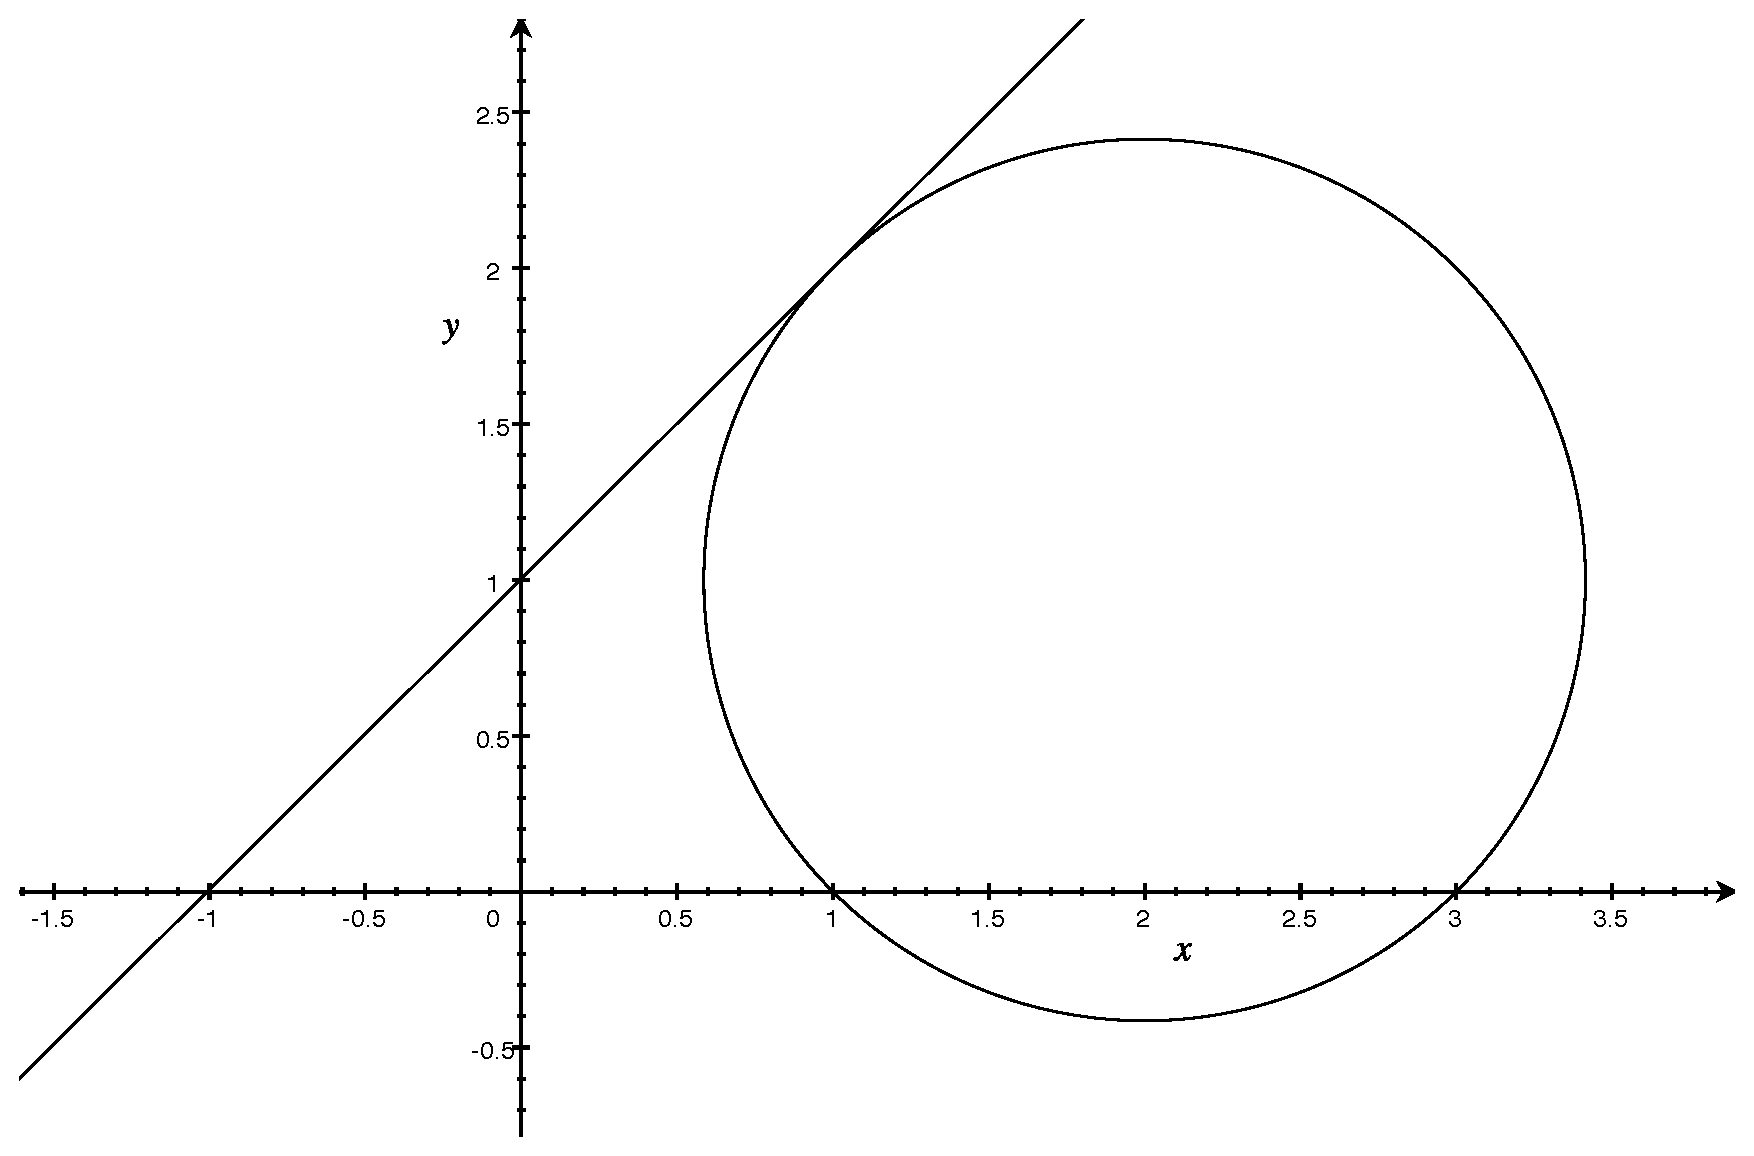
\includegraphics[height=7\baselineskip]{41.eps}
        \end{minipage}

        %|圆锥曲线|椭圆|12|向量|
        \section{已知$A$, $B$是由直线$x=\pm a$, $y=\pm b$所围成矩形相邻的两个顶点,点$P$是椭圆$\dfrac{x^2}{a^2}+\dfrac{y^2}{b^2}=1,(a>b>0)$上的任意一点,且存在实数$m,n$满足$\overrightarrow{OP}=m\cdot \overrightarrow{OA}+n\cdot \overrightarrow{OB} $,则$m+n$的取值范围是\3.}
        \lge{我们先进行一个仿射变换,令$x'=\dfrac{x}{a},y'=\dfrac{y}{b}$得到圆$C'$方程$x^2+y^2=1$,\\则$\xl{OP}=(cos\theta,sin\theta),m\cdot\xl{OA}=(m,m),n\cdot\xl{OB}=(n,-n)$,\\由$\overrightarrow{OP}=m\cdot \overrightarrow{OA}+n\cdot \overrightarrow{OB} $可得$m+n=cos\theta$.\\这样,由于三角函数的值域,答案就呼之欲出了.}

        \section{直线$l:y=kx+b$和椭圆$C:\dfrac{x^2}{4}+\dfrac{y^2}{2}=1$相交于$A,B$两点,按下列条件,求直线$l$的方程:\\(1)若$b=1$,$|AB|=\dfrac{4\sqrt{5}}{3}$;\\(2)若$b=1$,且直线$l$和$y$轴交于点$P$,满足$\xl{PA}=-\dfrac{1}{2}\xl{PB}$;\\(3)使线段$AB$被$M( \dfrac{1}{2},\dfrac{1}{2})$平分;\\(4)若以$AB$为直径的圆过原点,求$k,b$满足的等式.}


    \chapter{双曲线}
        \section{已知$l_1: y = x, l_2: y = -x$,动点$M(x, y)$,且$|x| > |y|$,记$M$到$l_1, l_2$的距离分别为$d_1, d_2$,满足$d_1 \cdot d_2 = \frac{a^2}{2}(a > 0)$.
        \\(1) 动点$M$的轨迹$\Gamma$的方程;
        \\(2) 若直线的方向向量为$(1, 2)$,过$(\sqrt{2}a, 0)$的直线$l$与$\Gamma$交于$A, B$两点,那么以$AB$为直径的圆是否恰过原点$O$?若是,求$a$的值;若否,判断原点在圆内还是圆外,说明理由.
        \\(3) 过原点$O$作斜率$k$为的直线交于$M$,$N$两点,设$P(0, 1)$,求$\triangle PMN$的面积$S$关于$k$的函数解析式,并求$S$的取值范围.
        }
        
        \begin{minipage}[b]{0.65\linewidth}
            \begin{enumerate}[(1)]
                \item \lge{由点到直线距离公式可得$d_1 = \frac{|x - 4|}{\sqrt{2}}, d_2 = \frac{|x + 4|}{\sqrt{2}}$, 代入$d_1 \cdot d_2 = \frac{a^2}{2}$中得$x^2 + y^2 = 1$.}
                \item \lge{设$l$的方程为$y = 2(2 - \sqrt{2}a)$,与$\Gamma$联立化简得$-3x^2 +8\sqrt{2}ax - 9a^2 = 0$, 由于$AB$是圆的直径,且$O$在圆上,所以设
                $\xl{OA} = (x_1, y_1), \xl{OB} = (x_2, y_2)$, $\xl{OA} \cdot \xl{OB} = 0$, 故$x_1x_2 + y_1y_2 = 0$. 由韦达定理得$x_1 + x_2 = \frac{8\sqrt{2}}{3}a$
                , $x_1x_2 = 3a^2$, $y_1y_2 = 4x_1x_2 - \sqrt{2}a(x_1 + x_2) + 2a^2$.于是得到$x_1x_2 + y_1y_2 = \frac{35}{3}a^2 = 0$,而$a = 0$与题意不符,故原点不在圆上.
                又$\xl{OA} \cdot \xl{OB} > 0$,故$<\xl{OA}, \xl{OB}> < \frac{\pi}{2}$.原点在圆外.}
                \item \lge{设$M(x_m, y_m), N(x_n, y_n)$,则$S_{\triangle PMN}  = \frac{1}{2} \cdot 1 \cdot |x_m| + \frac{1}{2} \cdot 1 \cdot |x_n| = \frac{1}{2}|x_m - x_n|$.
                设直线$y = kx + b$,与$\Gamma$联立得$(1 - k^2)x^2 - a = 0$, 又由韦达定理得$\frac{1}{2}|x_m - x_n| = \frac{1}{2}\sqrt{(x_m + x_n)^2 - 4x_mx_n} = \frac{a\sqrt{1-k^2}}{1-k^2}$,$k \in (-1, 1)$, $S \in [a, +\infty]$.}
            \end{enumerate}
        \end{minipage}
        \begin{minipage}[b]{0.25\linewidth}
            \centering
            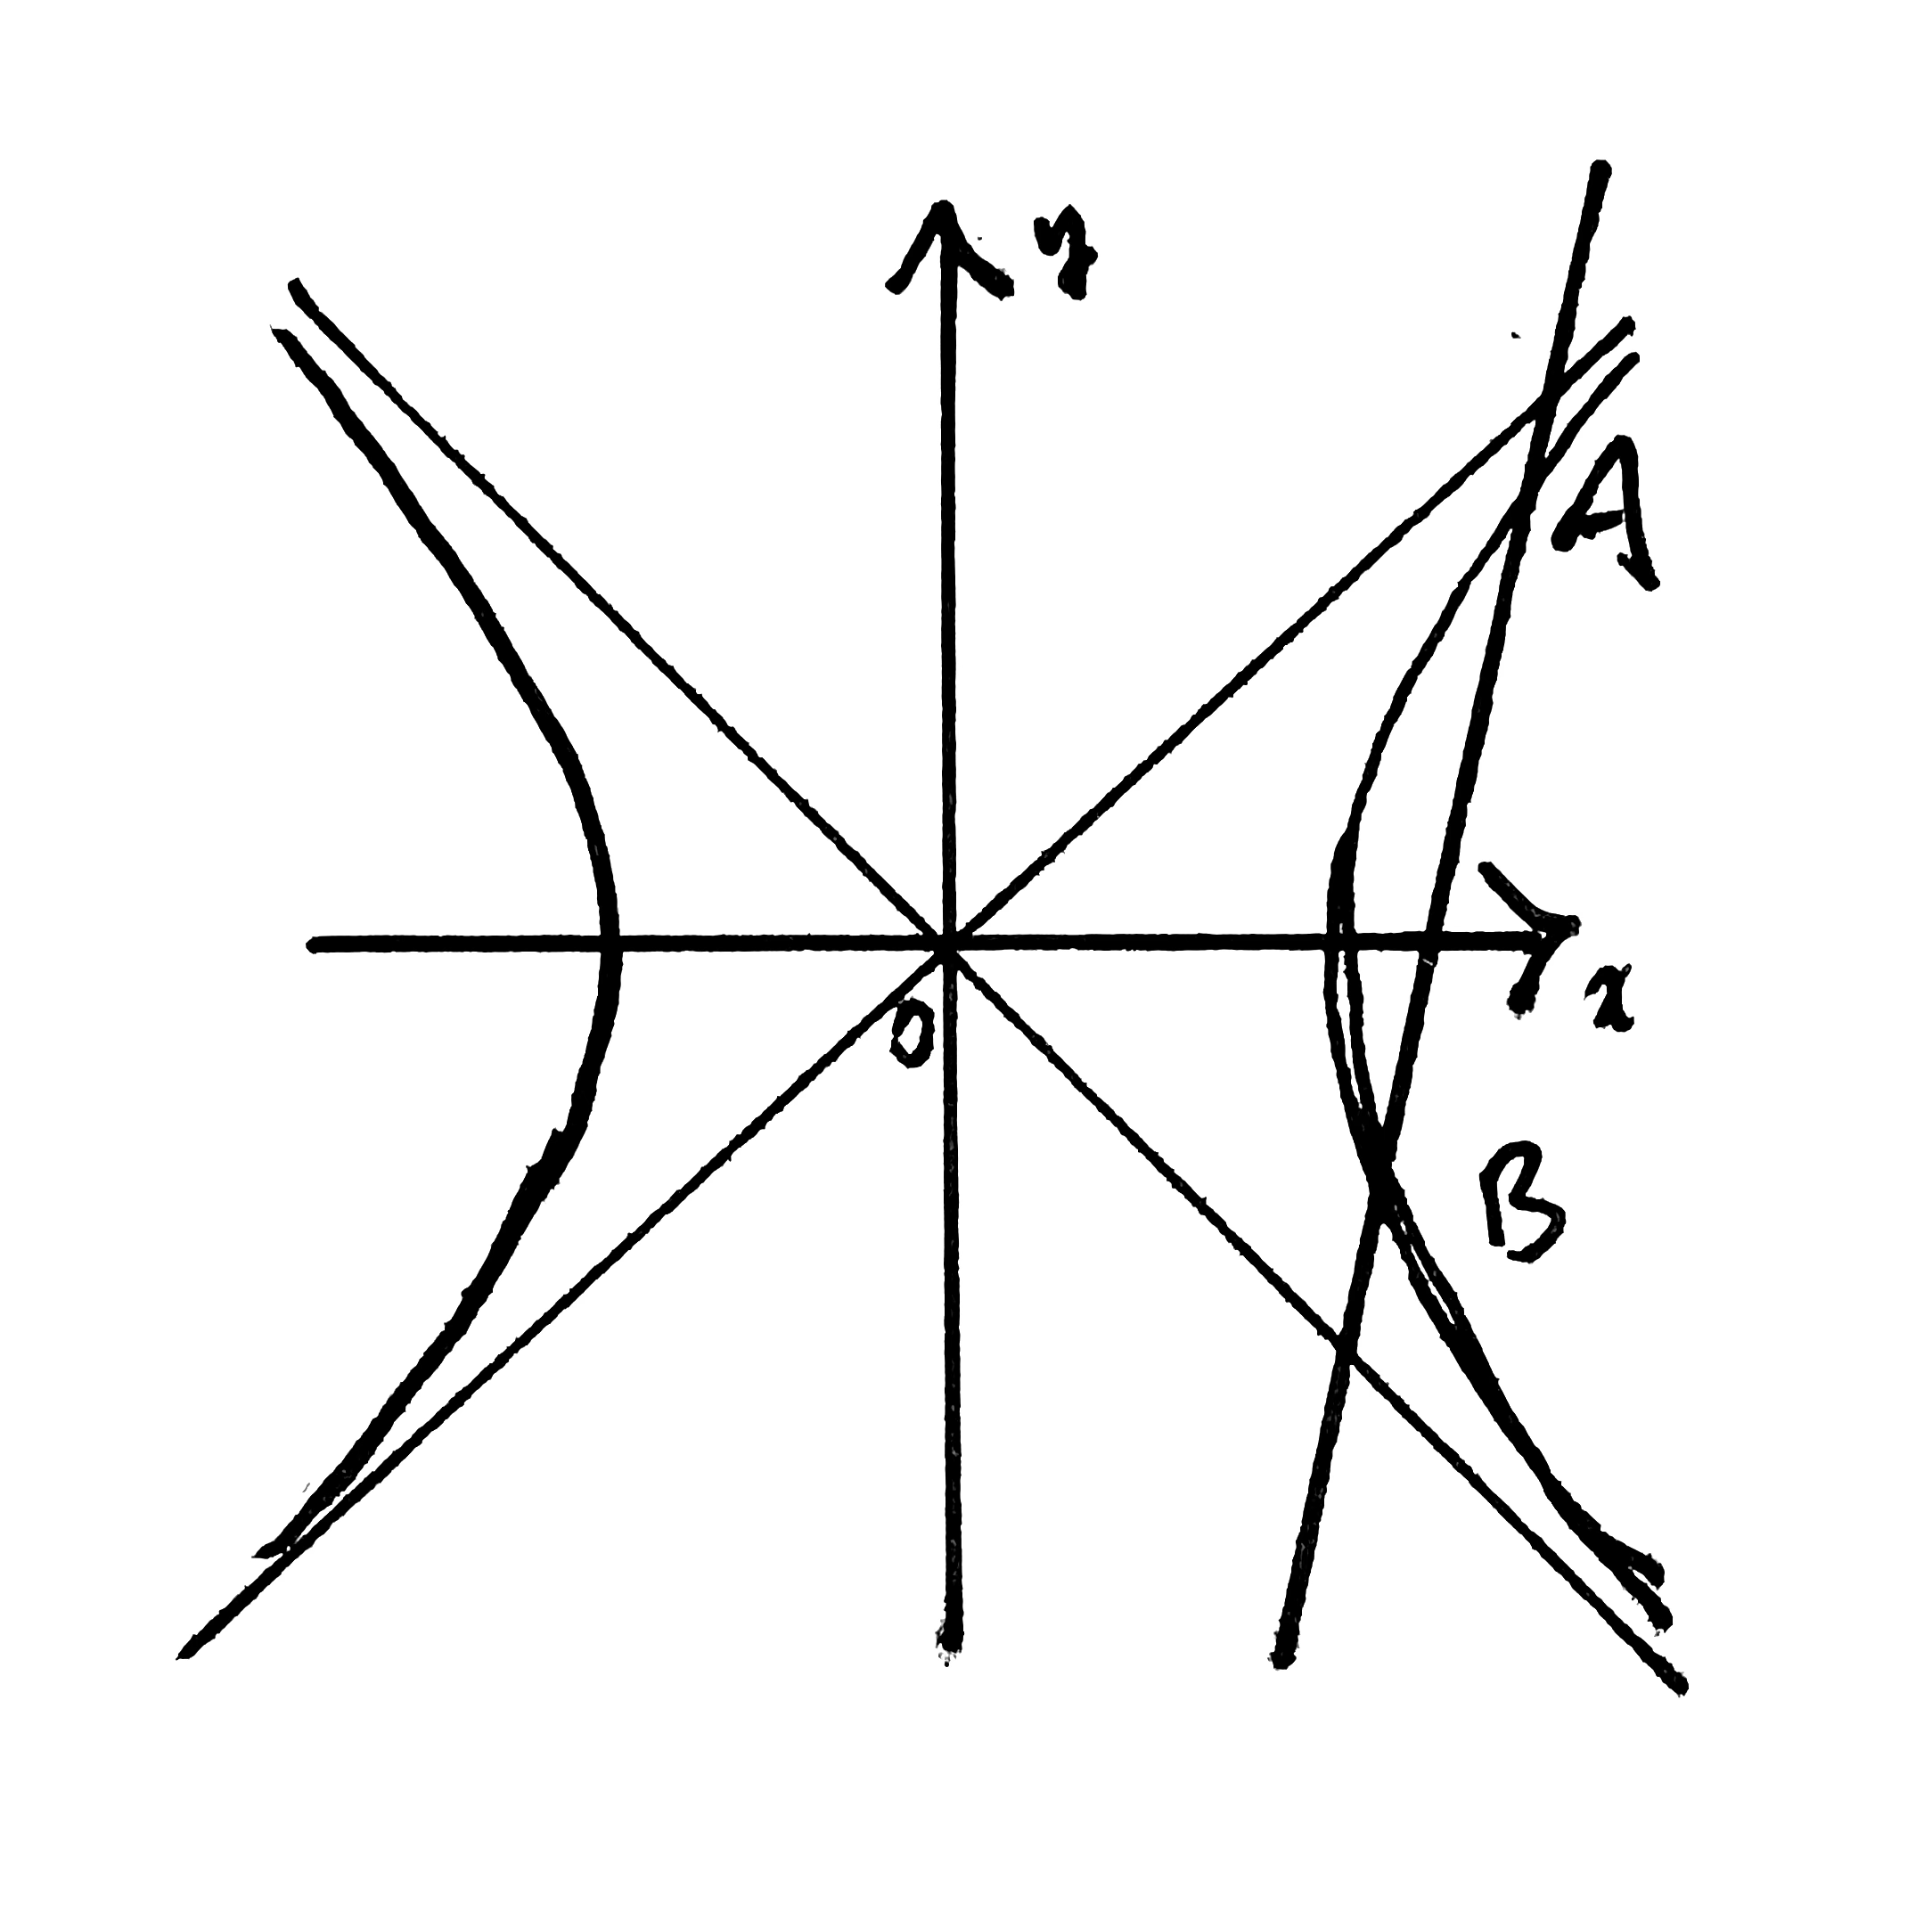
\includegraphics[height = 95pt]{2.png}
            \hfill
            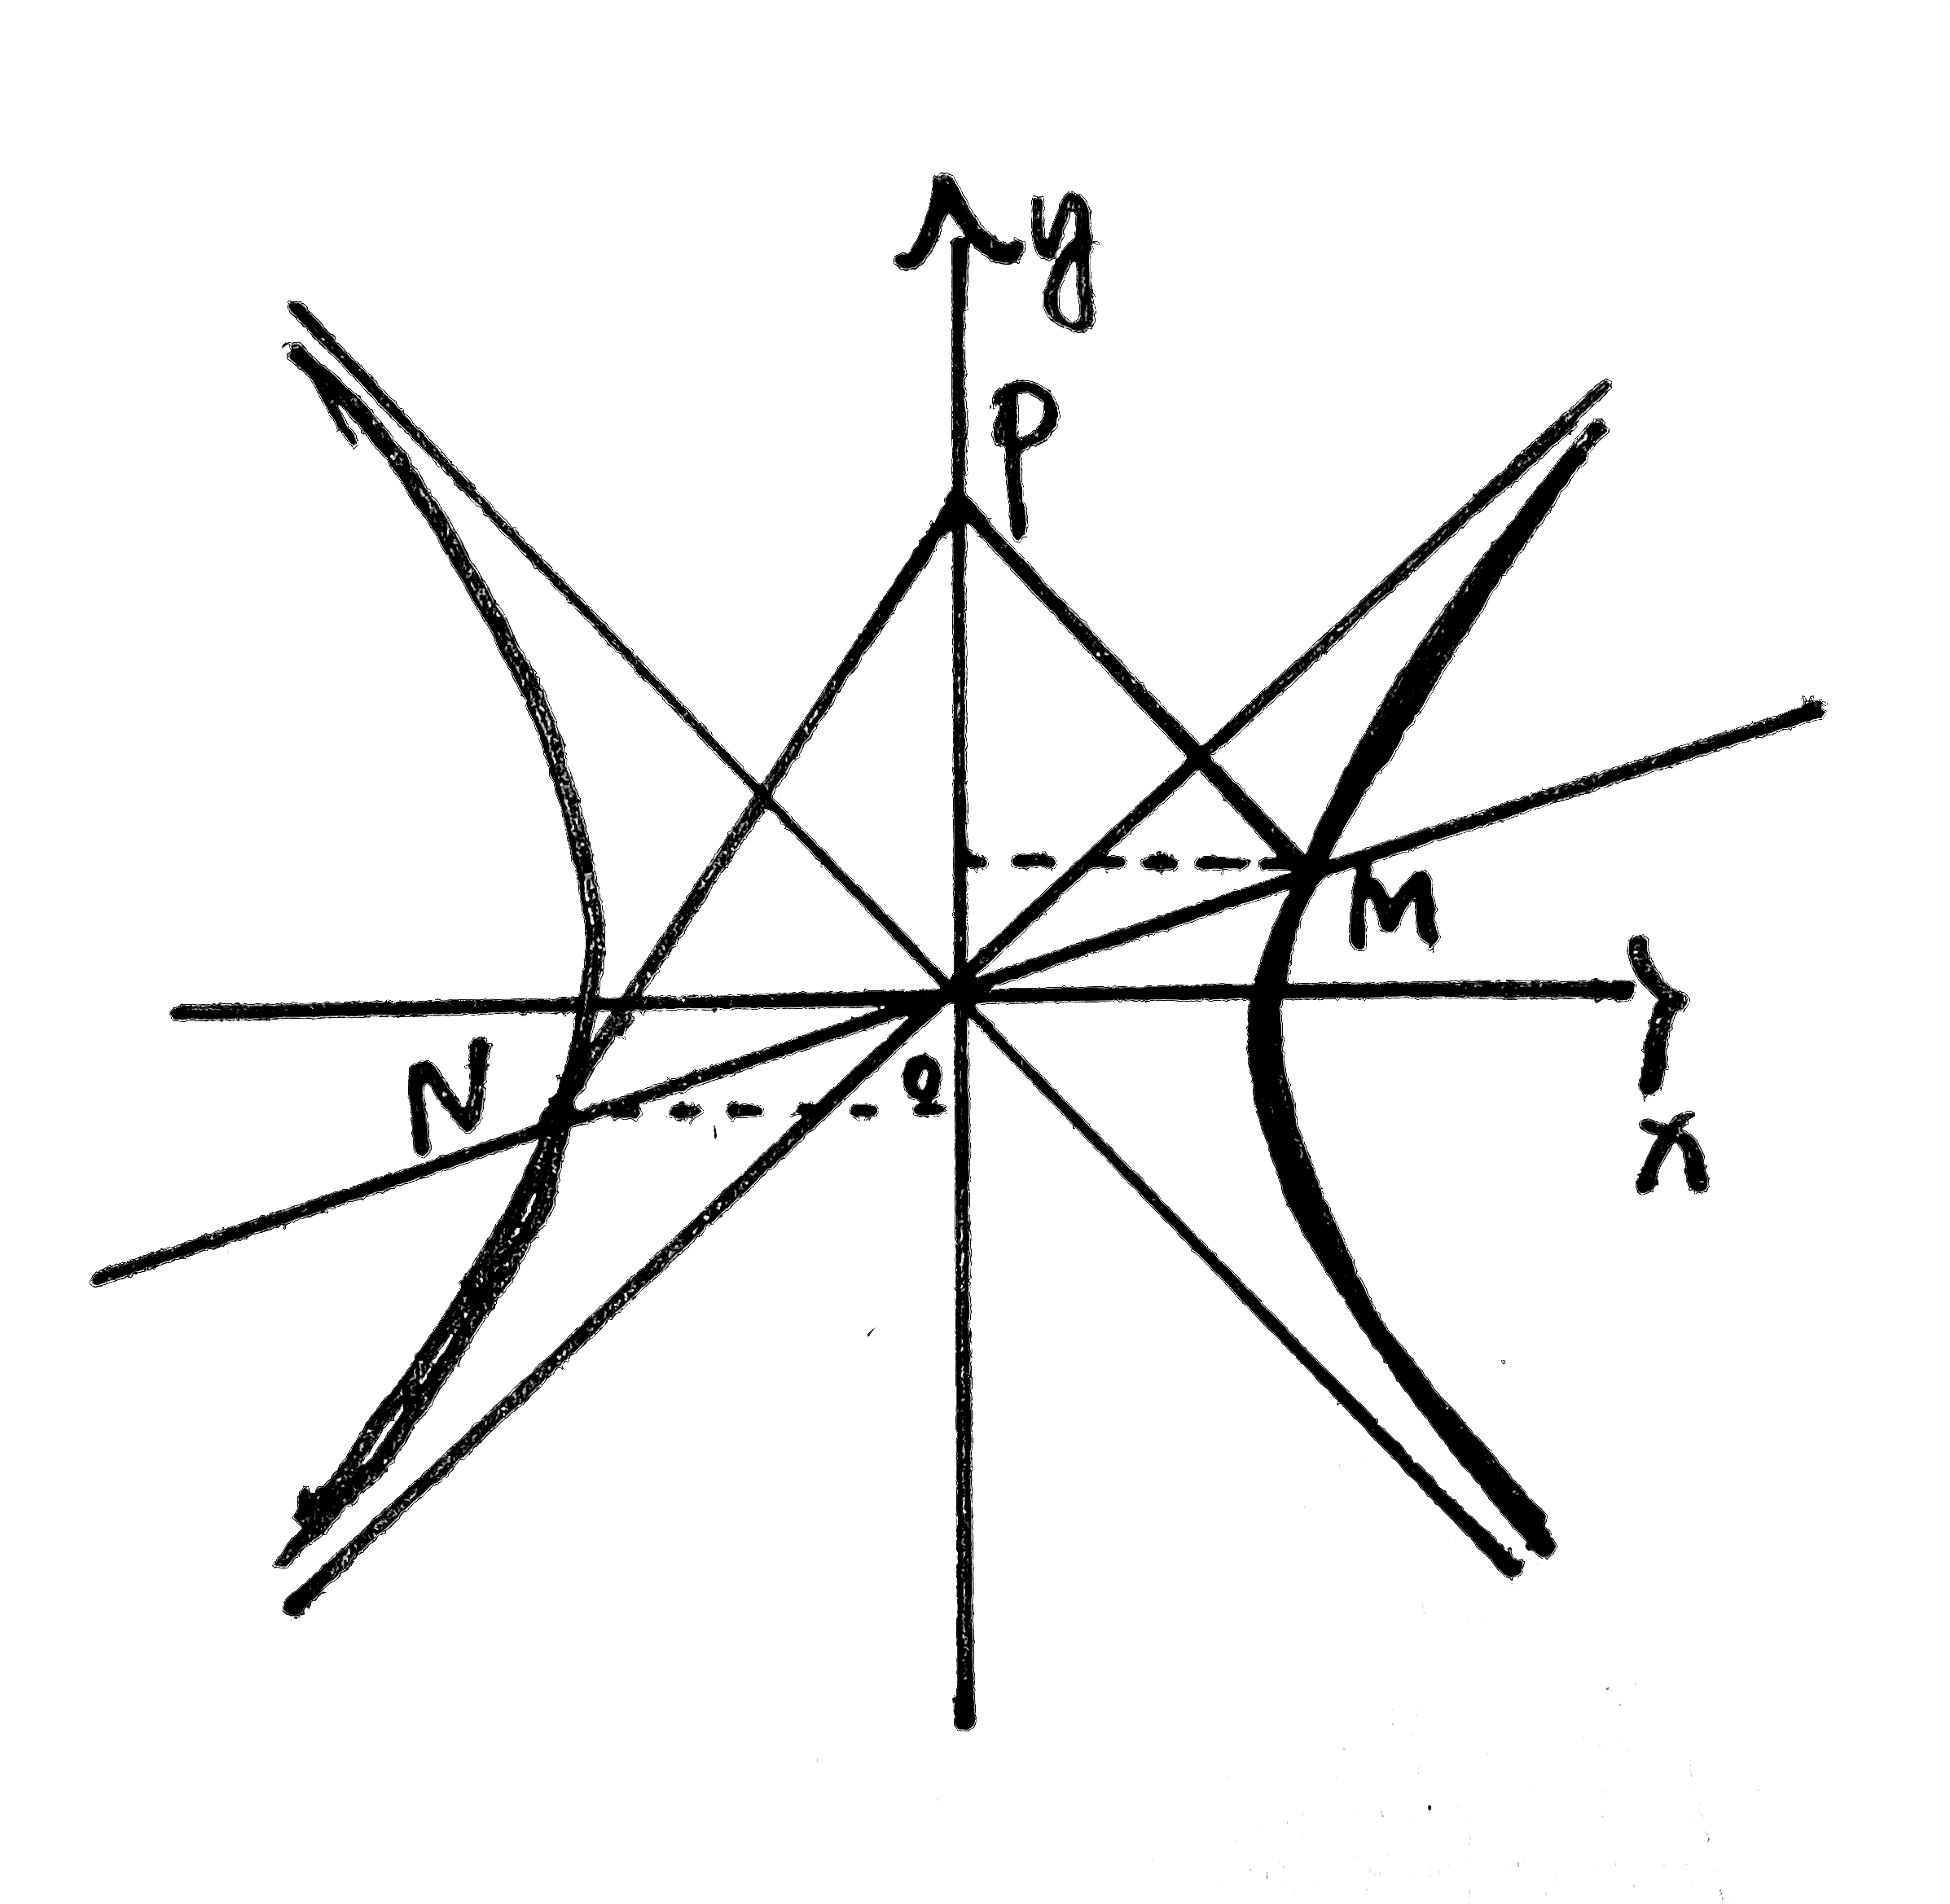
\includegraphics[height = 100pt]{3.png}
        \end{minipage}

    \chapter{抛物线}



\part{数列}

    %|数列|9
    \section{如果$f(n)=1+\frac{1}{2}+\frac{1}{3}+\cdots+\frac{1}{n}+\frac{1}{n+1}+\cdots+\frac{1}{2^n}(n\in \mathbb{N^*})$,那么$f(k+1)-f(k)$共有\2项.}
    \blk

    %|数列|12
    \section{首项不为$0$的等差数列${a_n}$前$n$项和是$S_n$,若不等式${a_n}^2+\dfrac{{S_n}^2}{n^2}\geq \lambda {a_1}^2$对任意$a_n$和正整数$n$恒成立,则实数$\lambda$的最大值为\2.}
    \blkc

    

\part{A}
    
    \section{当$x \in [a, + \infty)$时,幂函数$y=x^2$的图像总在$y=x^{\frac{1}{2}}$图像的上方,则$a$取值范围为\2.}
    \blkc
    
    \section{若对任意$x \in[1,2]$,均有$|x^2-a|+|x+a|=|x^2+qx|$,则实数$a$的取值范围为\2.}
    \blkc

    \section{四棱锥$P-ABCD$中,底面$ABCD$为直角梯形,$AD \pll BC, AB \perp BC,AB = AD,BC = 2AB,E,F$为$BC,BP$中点。\\ i、求证平面$AEF \pll $平面$DCP$; \\ ii、若$PBC \perp ABCD,AP$与$PBC$所成角为$45 °, CP \perp PB$,求$P-AB-C$大小。}
    \rightline{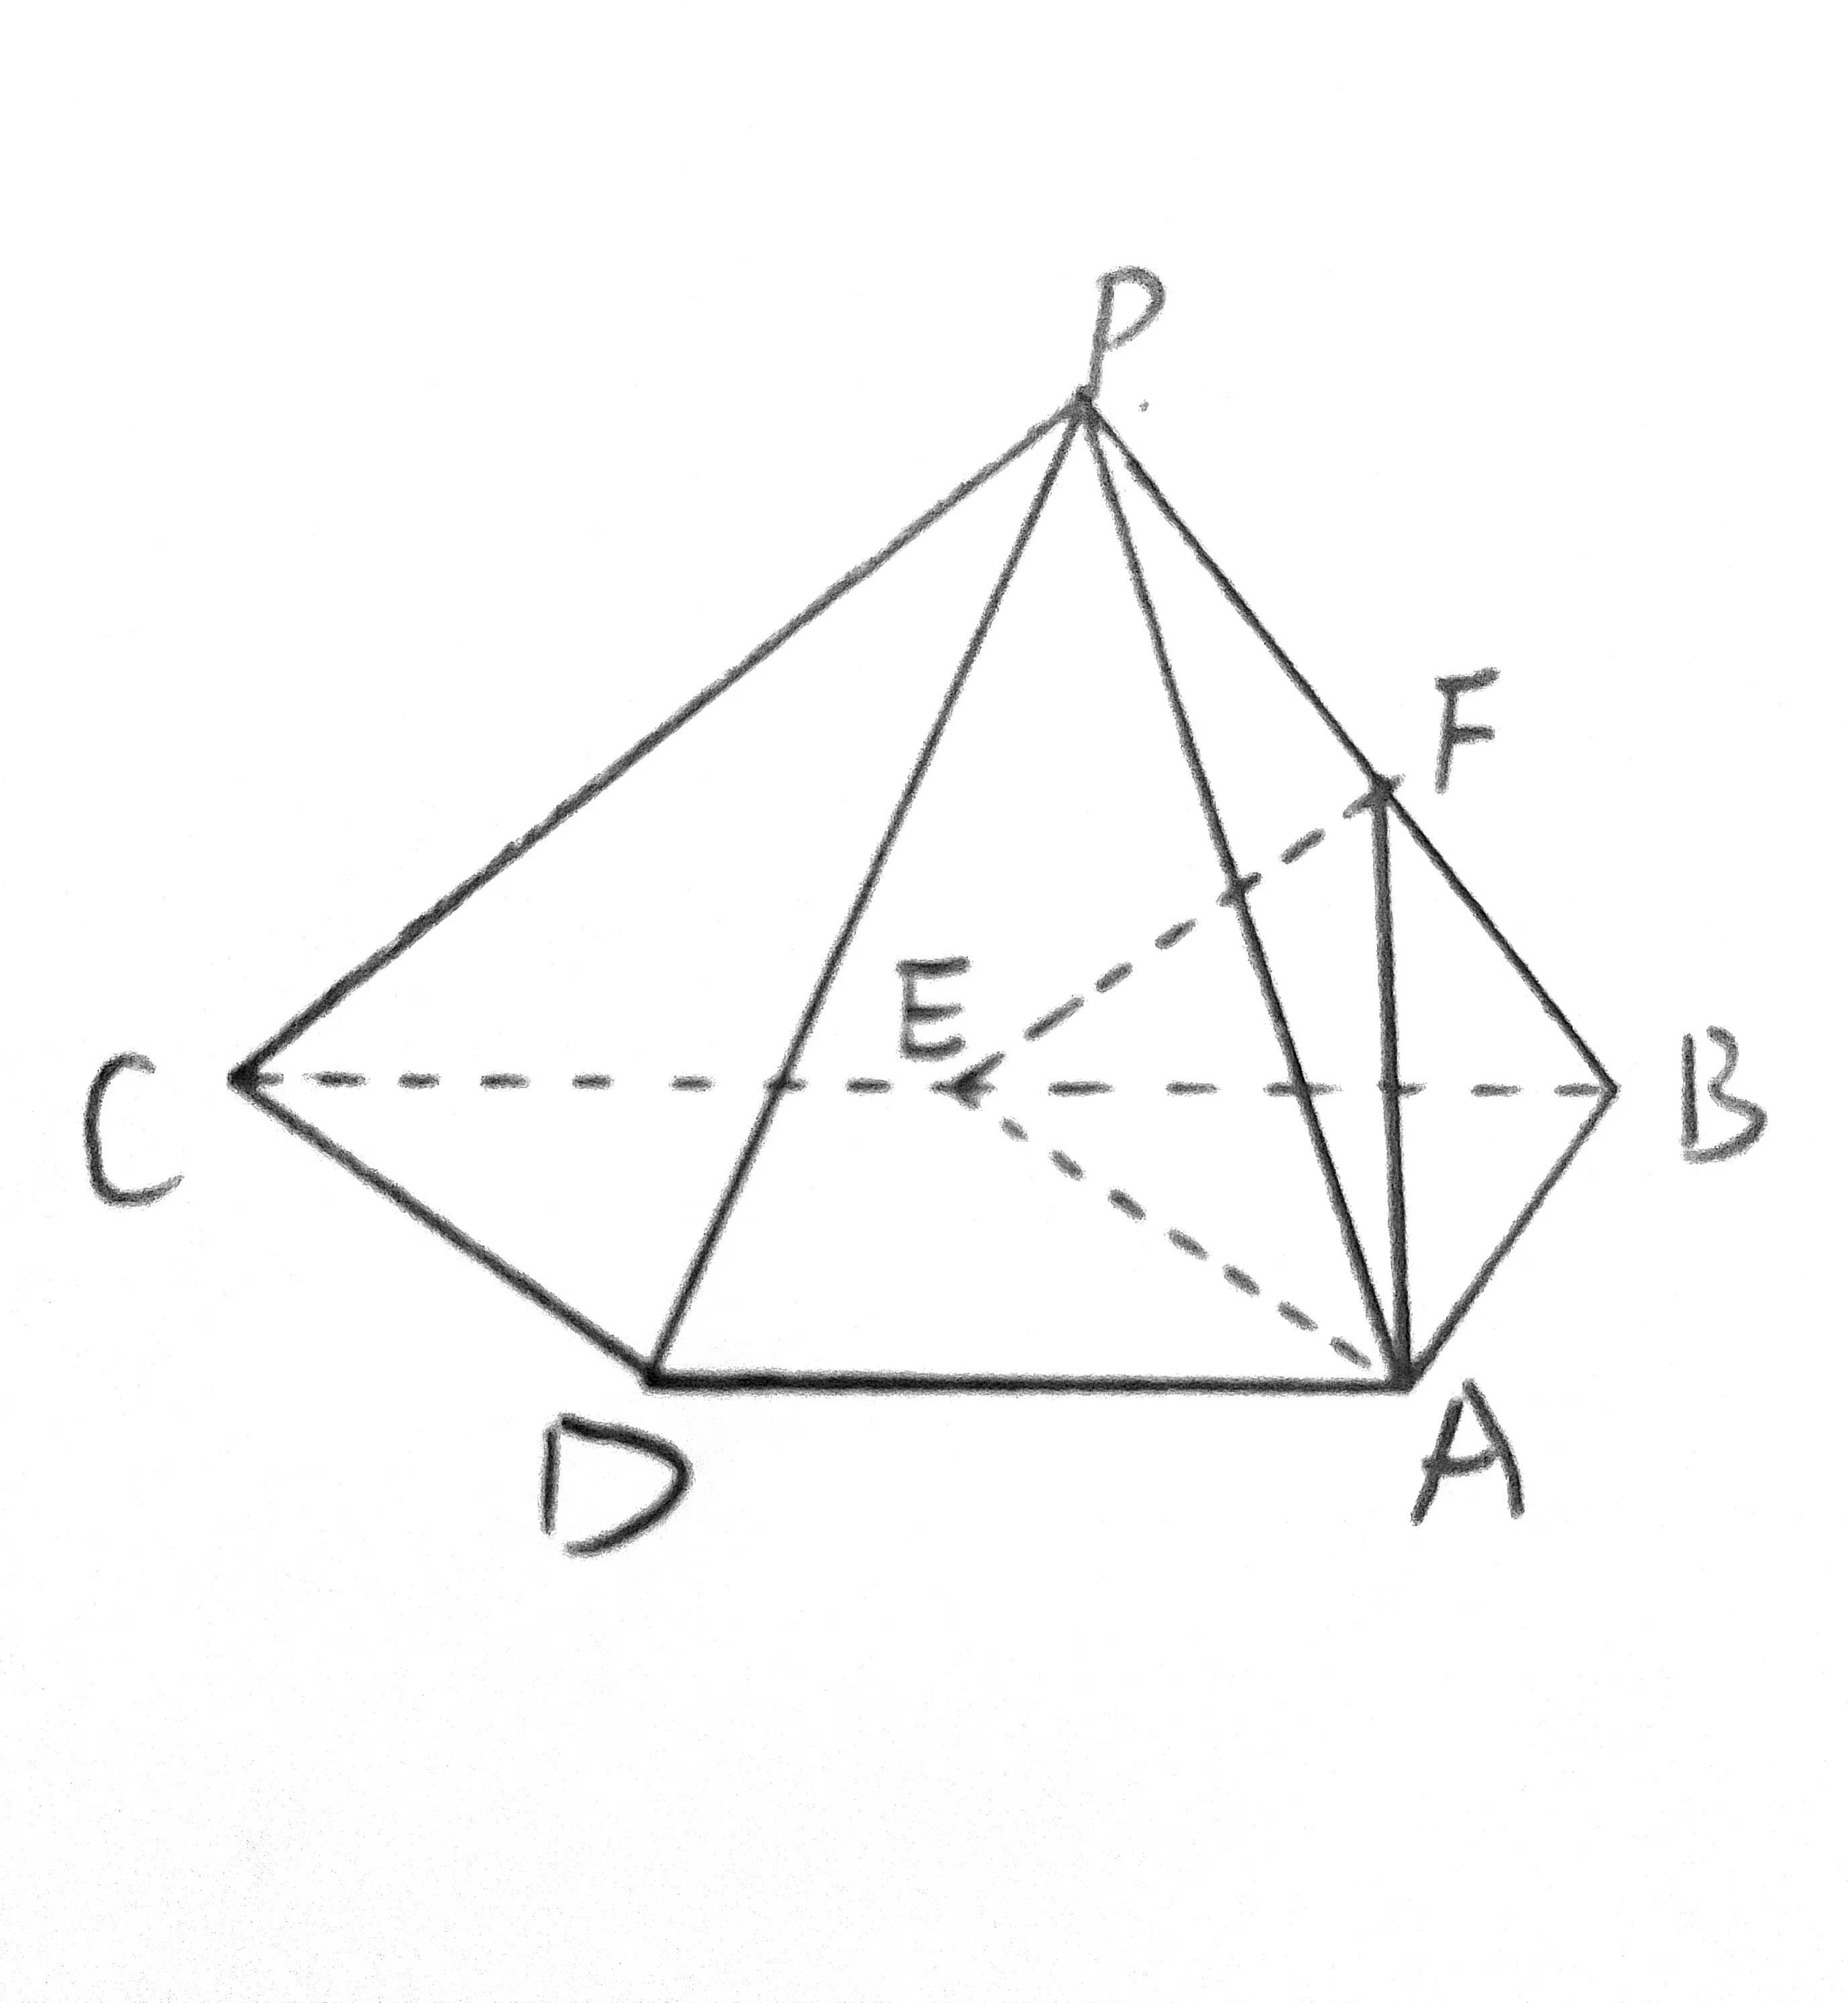
\includegraphics[height = 135pt]{5.jpg}}
    \blkc
    
    



\end{document}